\clearpage
\section{Measurements}
\label{sec:measurements}

In theory, it is possible to collect accurate data of Internet traffic
from a network. In reality, however, many issues confound such
measurements. Budget constraints driven by the cost of collection, or
the massive data storage facilities required due to the sheer amount
of data traversing a backbone network limit what can be achieved. And
even good measurement systems can suffer from errors and missing
data. Added to this, current operator practice rarely includes any
significant calibration of measurement apparatus, so often the degree
of accuracy of the measurements is unknown.

There are several well-known strategies for collecting traffic
measurements. A {\em packet trace} is a collection of packets headers
(perhaps with some payload) and timestamps.  A packet trace can be
collected through various means, for example, through hardware such as
a splitter placed strategically in optical fibre; adding a monitor
port on a router; or through software tools such as \texttt{tcpdump}
executed on several hosts in a shared network. An OD traffic matrix
can be constructed from such a trace by simple consideration of the IP
address in the packet headers (with the caveats mentioned earlier).

Such an approach is ideal in many respects: we have almost complete
information, and the matrices may be drawn at almost any time
resolution. However, collecting packet traces is expensive due to the
need for dedicated hardware, and the huge amount of storage required:
potentially, over a terabyte of data per hour on OC48 links (2.5 Gbps)
is needed. It is rare for any but the smallest network to be able to
completely instrument its network at this level of detail.

Fortunately, constructing a traffic matrix does not require such
detailed information. Perhaps the most common alternative is {\em
  flow-level aggregation} where packets are aggregated according to a
common flow key.  One popular definition of the key is the 5-tuple
comprised of the IP source and destination address, TCP/UDP source and
destination port numbers and protocol number. A series of packets
possessing a common key is called a \emph{flow}, and we maintain
simple statistics (byte and packet counters, and start and stop times)
for each flow. The aggregation of packets into flows reduces the
number of records needed to be stored by removing redundancies of data
from a packet trace. Flow-level collection is generally performed in
15 minute time bins\footnote{The issue of timing of flows is actually
  somewhat more complicated, but readers should refer to detailed
  descriptions of specific flow-capture protocols for information on
  their particular flow capture.} and is often an in-built function of
a router. The only additional infrastructure required is the Network
Management Station (NMS) and flow records themselves are usually
compressed by the router before being exported to the NMS. Despite
this reduction, flows arrive at a router at rapid rates and the
formation and storage of flow records at a router often burdens the
router's CPU.

To further reduce the number of flow records at a router, sampling
methods are employed. The most popular sampling method is packet
sampling, where incoming packets are sampled based on predetermined
sampling patterns, used, for instance by Cisco's NetFlow
\cite{NetFlow}. Such pseudo-random patterns have a similar effect to
independently picking incoming packets given sufficient mixing of
traffic.  The sampling rates can be adjusted depending on the capacity
of the incoming links with recommendations such as 1 in 256 packets
for OC192 links (10 Gbps). Higher capacity links require aggressive
data reduction, and so lower sampling rates are used.

Packet sampling reduces the number of flows significantly by omitting
many, but it is important to realise that although it may select
\emph{packets} in an unbiased way, it is not unbiased with respect to
\emph{flows}. Packet sampling has a strong bias towards long flows,
since it is more likely to have sampled packets from a long flow than
a short one. Furthermore, the sampled flow size is not the true size
of the flow and there are several works
\cite{Duffield05Sampled,Duffield05Smart} proposing methods to sample
and estimate the true size of a sampled flow. While the strong bias
may be a problem for some applications, there is usually no problem in
using sampled flows to form the IE traffic matrix.

In addition to packet sampling, we may also sample a set of flows, and
these sampled flows can then be used to create traffic matrices. The
resulting reduction in intermediate storage and processing can be
substantial, particularly if the sampling is done in a clever way
\cite{Duffield05Sampled,Duffield05Smart}.

It must be remembered that sampling is an inherently lossy process,
regardless of the underlying sampling method used.  The loss of
information translates into errors or noise in the data. The size of
these errors should, in best practice, be estimated for a given setup,
but most operators do not undertake such procedures due to the
difficulties involved in obtaining ground-truth data with which to
compare to the sampled data. In many cases it is simply assumed that
these errors, once the data is aggregated further into traffic
matrices, are negligible, but this assumption is rarely validated.

Furthermore, there is the problem of possible multiple counting of 
traffic flows from the aggregated records of flows. The problem 
arises if the aggregated flow records come from internal backbone
routers of the network, since a single flow may be recorded more than
once by several routers if it traverses several links. One way to
get around this relies on the placement of the measurement
points. One simply performs traffic measurements at the ingress points.
Specifically, the measurements are performed on the backbone routers 
connected to the access routers, or on dedicated devices placed at the 
links connecting the access routers to the backbone routers. 
In this way, the total incoming traffic of the network may be reliably
measured from the flow records. There is then no longer a problem of 
multiple counting of flows.

Trajectory sampling \cite{Duffield01Trajectory,Duffield04Unreliable} 
is another method. It exploits the pseudorandomness 
of a hash function to simulate random sampling of packets. However, if a flow 
was sampled at one router, it will be consistently sampled at every 
other router the flow traverses by the deterministic operation of hash 
functions. Since the tracking of flows is now feasible, it is then also 
straightforward to disambiguate their identities and eliminate multiple
counting. The downside is that a network operator must deploy 
trajectory sampling throughout the whole network, and configure
the hash function on each router each time before a measurement interval
begins.

A less costly alternative is easily obtainable link counts. A link
count, or link load measurement, gives the volume (in bytes or
packets) of traffic on a link during a particular time interval.  Link
counts are obtainable from measurement data by the Simple Network
Management Protocol (SNMP) \cite{SNMP}, defined as part of the IETF
standard and present on many Internet devices, including most
routers. SNMP data from a single router provides two measurements for
each interface, the incoming and outgoing byte counts. SNMP data is
obtained by an NMS by periodically polling requests through an
interface, typically UDP port 161. The polling period varies from 1
minute to several minutes, but the default seems to be 5 minutes. SNMP
data is highly susceptible to error, due to the following factors:
\begin{enumerate}
\item \textbf{missing link observations}: data is transmitted via
  unreliable UDP packets and there may be errors when copying the data
  into the observer's archive, 

\item \textbf{incorrect link observations}: poor router vendor
  implementations causes inaccuracies, and

\item \textbf{sampling coarseness}: polling times are often inaccurate
  either due to poor NMS or SNMP agent implementations, high loads, or
  network delays.

\end{enumerate}
As with flow-level data, link count data should be calibrated, but
rarely is. There is only one experiment of which we are aware that
does so \cite{roughan10:_case_accur_snmp_measur}. The study showed
that in one network, SNMP errors were typically low (90\% of
measurements had an error of less than 1\%), but a small number of
measurements were very large, some as large as 100\%. This type of
heavy-tailed distribution causes problems for some estimation
approaches and should be considered in context.

Another drawback of SNMP data is that it only provides aggregate link
statistics, omitting details such as types of traffic on the link and
the traffic source and destination. Despite all these issues, SNMP
data is, at present, the easiest and perhaps most common way to obtain
large-scale traffic data.

The observed link counts provide some information about the traffic
matrix, but only in an indirect manner. Thus, the traffic matrix has
to be inferred through a process called \textit{tomography}. 
Network tomography was first introduced by Vardi
\cite{Vardi96Tomo}, with the inspiration taken from inference
techniques for medical tomography as both problems are similar in
nature. Vardi's work was subsequently expanded upon by Tebaldi and
West \cite{Tebaldi98Tomo} and Cao \etal\cite{Cao00Tomo}. Various
other works in network tomography measure other properties of the
network, such as link delays (see
\cite{tomo_CCLNY_2004,tomo_CHNY_2002} for an overview) via active
packet probing, but for traffic matrix estimation, we are only
concerned with the link count observations from SNMP data.

Mapping traffic to links requires topological and routing data in the
form of a \emph{routing matrix}. The routing matrix $\bA$ is defined
by
\begin{align*}
A_{i,r} = 
\begin{cases}
F_{i,r}, & \text{if traffic for $r$ traverses link $i$},\\
0, & \text{otherwise}.
\end{cases}
\end{align*}
where $F_{i,r} \in (0,1]$ is the fraction of traffic from
source-destination pair $r = (s,d)$ traversing link $i$. Fractional
values occur in cases when load balancing is used, but it has often
been assumed that $F_{i,r} = 1$, resulting in $A_{i,r} \in
\{0,1\}$. The size of the routing matrix depends on the network: with
$N$ nodes and $L$ links, the routing matrix has size $L \times N(N-1)$
(traffic from a node is assumed not rerouted to itself).

Information on the routing matrix can be obtained from several
different sources (router configuration files, traceroutes, or from
the routing protocols themselves), but the collection of such
information is not the topic of the chapter. The interested reader is
referred to \cite{Feldmann00Netscope,Feldmann01TMdemand}.  

A common assumption is that the routing matrix remains stable during
the measurement interval, thus the temporal dependence is dropped,
\ie~$\bA(t) = \bA$ for all $t \in \cT$. However, changes in routing
may occur if there are link or router failures, necessitating traffic
reroutes. Generally, it is assumed the measurement interval is chosen
over a period of time (minutes to hours) when $\bA$ is stable enough
to be considered static, justified by observations in
\cite{Paxson97Routing}, however in at least one case it is proposed
that the changes be created, and
exploited~\cite{soule07:_estim_dynam_traff_matric_using} for traffic
matrix inference.


\begin{figure}[!thbp] 
  \begin{center}
    \hfill
    \begin{subfigure}[b]{\twoup}
      \centering
      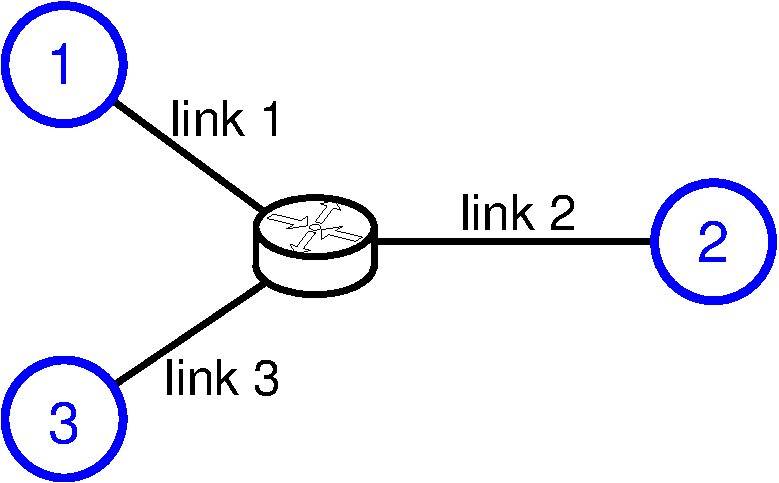
\includegraphics[width=1\columnwidth]{tm_formulation.pdf}
      \caption{Link labels}
      \label{fig:tomo_a}
    \end{subfigure}
    \hfill
    \begin{subfigure}[b]{\twoup}
      \centering
      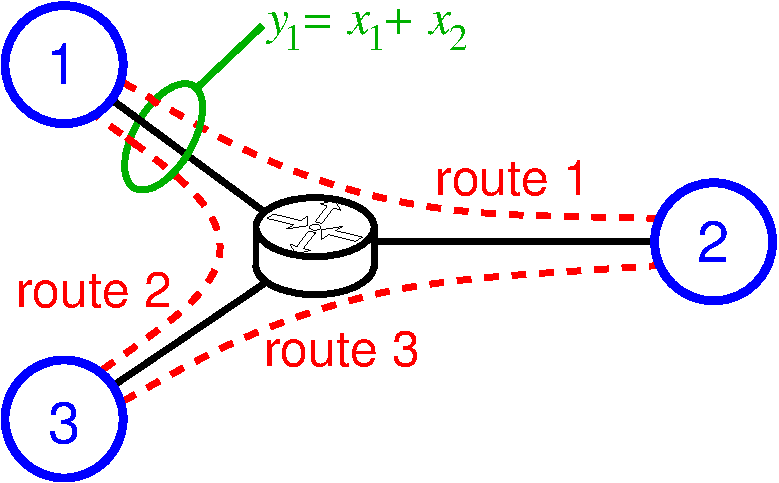
\includegraphics[width=1\columnwidth]{tm_formulation_2.pdf}
      \caption{Traffic labels and routes}
      \label{fig:tomo_b}
    \end{subfigure}  
    \hspace*{3mm}
    
    \caption{A simplified network and traffic (the main
      simplifications are that we only consider a single router, and
      only consider unidirectional traffic, not bidirectional as in
      real networks).\label{fig:tomo}}
  \end{center}
\end{figure}         

All the link counts may be grouped into an $L \times 1$ vector
$\by$. Then, based on link observations in one measurement interval,
the SNMP link counts may be expressed as 
\be 
  \by = \bA \bx,
  \label{eq:observation}
\ee 
where $\bx$ is the $N(N-1) \times 1$ vectorised version of the
traffic matrix $\bX$, with its columns stacked upon one another.  

\autoref{fig:tomo} presents an example of \autoref{eq:observation}. It
shows how the traffic on a single link $y_1$, is built from the sum of
traffic routed across the link $x_1 + x_2$. We can see that by
stacking each of these equations we would get
\be
  \left(\begin{array}{l} y_1 \\ y_2 \\ y_3 \end{array} \right) =
  \left(\begin{array}{lll} 1 & 1 & 0 \\ 1 & 0 & 1 \\ 0 & 1 & 1 \end{array} \right)
  \left(\begin{array}{l} x_1 \\ x_2 \\ x_3 \end{array} \right),
\ee
which, written in matrix notation, is just
\autoref{eq:observation}. Note that in this case the routing matrix
$\bA$ is invertible, so the problem of inferring the traffic matrix from
link measurements is easy, but this is rarely the case. Usually, $L$
is usually much smaller than $N(N-1)$, and so the
problem is highly underconstrained.

There are two main assumptions implicit in this observation model. It
assumes the traffic matrix is stationary, \ie~its statistical
properties remain stable throughout the measurement interval and there
are no errors in the measurement. Stationarity is preserved by
choosing an appropriate measurement interval, say 1 hour (see
\autoref{sec:models}). Moreover, in reality, errors do occur and to
account for it, the model \autoref{eq:observation} is extended to 
\be 
\by = \bA \bx +\bz.
 \label{eq:observation_noise}
\ee 


\noindent The second model is a simple noise additive model often used
to test the robustness of an inference technique. Each element of the
additive noise term $\bz$ is typically chosen to be independent and identically
distributed (i.i.d.) white
Gaussian noise with mean zero and variance $\sigma^2$. Often
$\sigma^2$ is kept small, as large values would result in some
elements of $\by$ violating the non-negativity constraint. It is
for this reason other distributions may be used, for example,
log-normal or gamma distributions. Additionally, due to the problem of
missing link information due to poor SNMP implementation, some of the
elements of $\by$ may be missing. Finally, if the given routing
matrix $\bA$ is incorrect, the observations $\by$ would
significantly depart from the true SNMP link counts. However, most
works assume an accurate $\bA$ because there are reliable methods for
obtaining routing information \cite{Shaikh02OSPF}.

There are usually many less links than the total number of IE pairs,
and so the inverse problem above is highly underconstrained.  Whether
noise is present or not there may be an infinite number of solutions
$\bx$ that fit the observations
\eqref{eq:observation}. \autoref{fig:tomo_hard} shows a picture of
such a network, where we only measure at the bottleneck. Now, even in
this very simple network the equations $y_1 = x_1 + x_2$ are
underconstrained. In order to make progress, some additional
information needs to be assumed, usually in the form of a traffic
matrix model, and we shall consider some of these in the following
section.



\begin{figure}[!thbp] 
  \begin{center}
    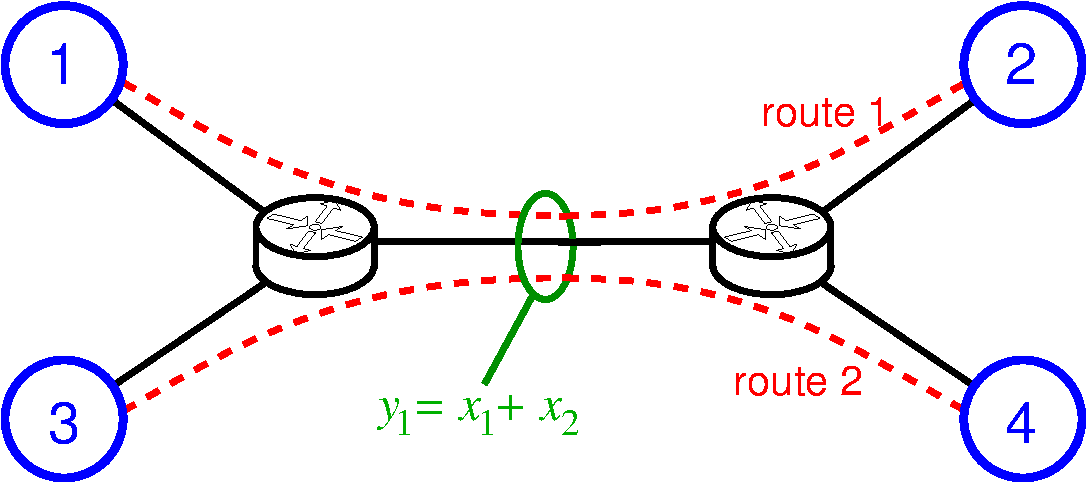
\includegraphics[width=0.6\columnwidth]{underdetermined.pdf}
    \caption{A harder inference problem where we only have one
      measurement, but two traffic elements to estimate. There is
      therefore a fundamental ambiguity in this problem.
      \label{fig:tomo_hard}}
  \end{center}
\end{figure}         

Before moving on to the modelling aspects of traffic matrices, note that
there are other strategies for measurement. For instance, if MPLS is
being used, this creates a set of tables (in many implementations)
that can almost be read directly to obtain the matrix (\eg~see
\cite{blili08:_best_pract_deter_traff_matric}).  Alternatively, the
network operator may have more accurate local traffic matrices,
obtained through specific functionality at the routers. It is, in
principle, easy for a router to keep counts of its decisions
\cite{Varghese03Measure}, essentially amounting to a table of the
volumes of traffic between pairs of interfaces.  Locality here is
defined in the sense of the matrix's restriction to a single router --
we essentially see an IE traffic matrix of the single router's
interface.  These local matrices from all routers in the network can
be used to improve the estimation of the IE traffic matrix; see
\autoref{sec:applications}. On some special cases, such as a star
network, a single local matrix would be equivalent to the traffic
matrix, serving to highlight the information gain from local traffic
matrices. These matrices provide greater than a two-fold increase in
accuracy of the tomography estimation schemes by
\cite{Medina02TMdirections,Zhang03Fast}.

